\documentclass[12pt, a4paper]{article}
\usepackage[utf8]{inputenc}
\usepackage[T1]{fontenc}
\usepackage[spanish]{babel}
\usepackage{amsmath, amssymb}
\usepackage{graphicx}
\usepackage{booktabs}
\usepackage{hyperref}
\usepackage{cite}        % o biblatex según prefieras
\usepackage{siunitx}     % unidades SI en minúscula, obligatorio por rúbrica
\usepackage{float}
\usepackage{caption}
\usepackage{graphicx} % Required for inserting images
\usepackage{tikz}
\usetikzlibrary{shapes.geometric, arrows.meta, positioning}
\usepackage{svg}
\usepackage{subcaption}

\title{Proyecto 1-ACSS}
\author{
Renato Bedriñana Cárdenas,
Dennis Huaman Yrigoin
}
\date{May 2026}

\begin{document}

\maketitle

% ==========================================
% SECCIONES DEL INFORME

% ==========================================

\section{Introducción y Objetivos}
El sistema diseñado permite medir la masa de recipientes de hasta
\SI{1.5}{\kg} mediante una célula de carga resistiva de aluminio de
\SI{5}{\kg} de capacidad nominal \cite{loadcell_datasheet}.
La señal diferencial generada por el puente de Wheatstone se
acondiciona, digitaliza y procesa para obtener una lectura estable
en gramos.

% (excitación -> sensor -> filtro RFI -> AD623 -> DAQ -> LabVIEW)
\begin{figure}[H]
    \centering
    %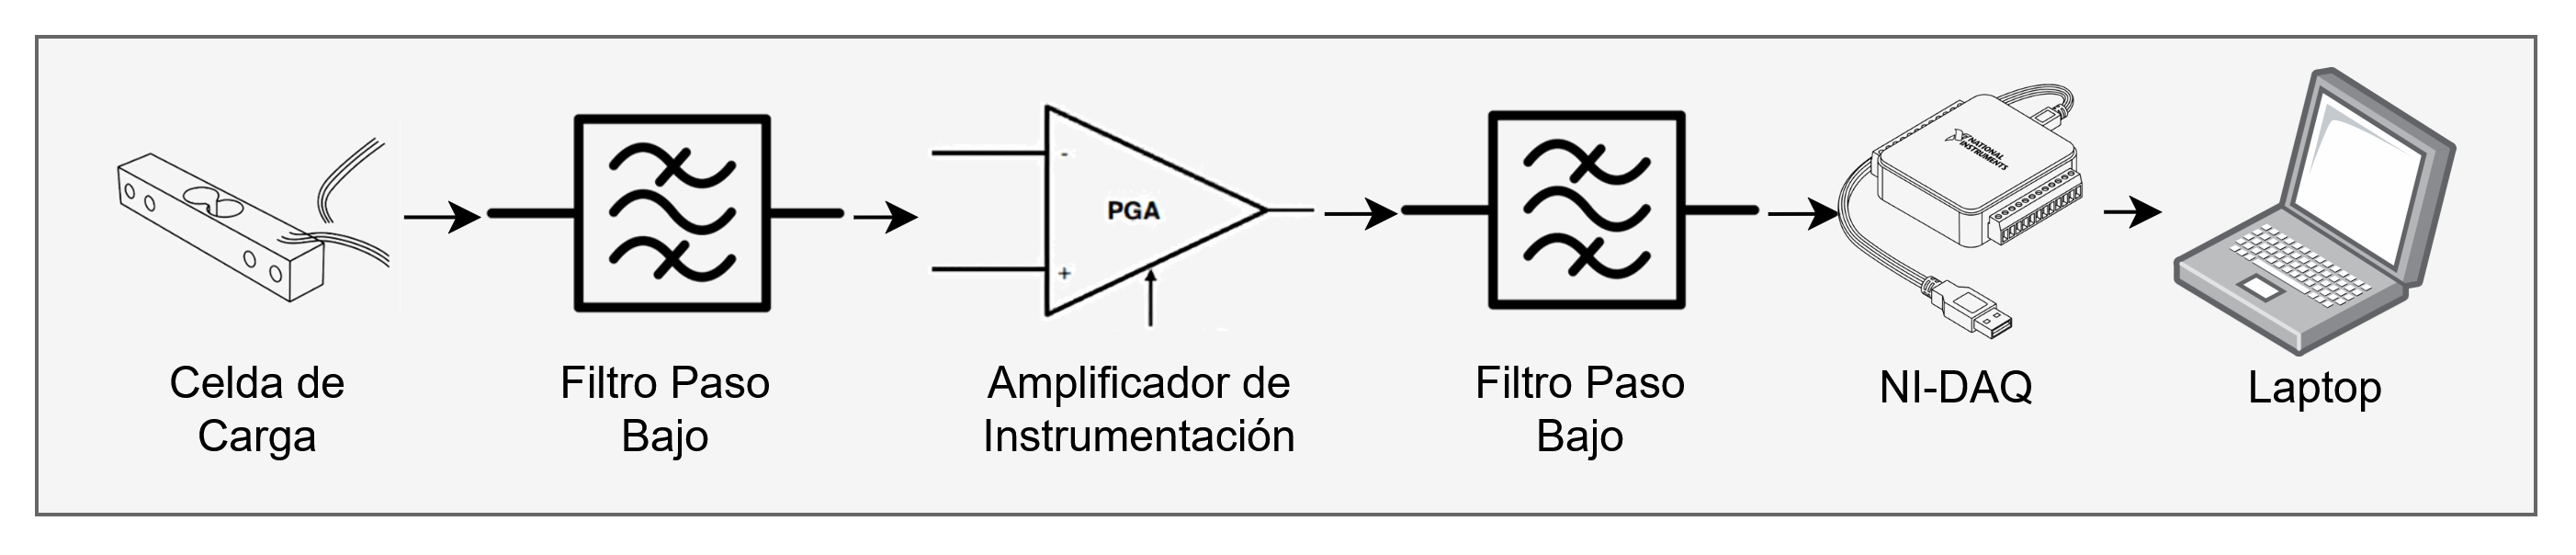
\includegraphics[width=0.85\textwidth]{figs/diagrama_bloques.png}
    \caption{Arquitectura general del sistema de pesaje a nivel de bloques.}
    \label{fig:bloques}
\end{figure}

\subsection{Objetivos}

El objetivo principal consiste en diseñar, montar y verificar una
báscula de precisión orientada al pesaje estático. De forma más
específica, se persigue:

\begin{itemize}
    \item Dimensionar analíticamente cada etapa del acondicionamiento
          de señal.
    \item Garantizar márgenes de seguridad frente a la saturación
          del amplificador.
    \item Validar el modelo matemático con medidas reales en la
          \textit{protoboard}.
\end{itemize}

\subsection{Requisitos técnicos}

\begin{itemize}
    \item Rango de pesaje: de \SI{0}{\g} a \SI{1500}{\g}.
    \item Tensión de excitación estable de \SI{4.096}{\V}
          (MCP1541) \cite{microchip_mcp1525_2012}.
    \item Pedestal de referencia de \SI{1.0}{\V} para evitar
          saturación por desequilibrio negativo (MCP6021) \cite{mcp6021_datasheet}.
    \item Frecuencia de corte del filtro diferencial RFI próxima
          a \SI{5}{\Hz}.
    \item Adquisición en modo diferencial en la NI USB-6001
          \cite{ni6001_datasheet}.
\end{itemize}

\section{Acondicionamiento Estático (Análisis DC y Amplificación)}
\subsection{Generación de la tensión de excitación}

Se emplea la referencia MCP1541 para proporcionar una excitación estable de \SI{4.096}{\V} al puente de Wheatstone, con una tolerancia de \(\pm\SI{0.1}{\percent}\) y un coeficiente de temperatura de \SI{50}{ppm\per\celsius} \cite{mcp6021_datasheet}. El circuito incorpora dos condensadores de desacoplo en el pin de salida para atenuar transitorios y ruido de alta frecuencia.

\begin{figure}[H]
    \centering
    \begin{subfigure}[b]{0.48\textwidth}
        \centering
        %\includesvg[width=\textwidth]{figs/CKTO VREF}
        \caption{Esquema del circuito.}
        \label{fig:vref_esquema}
    \end{subfigure}
    \hfill
    \begin{subfigure}[b]{0.48\textwidth}
        \centering
        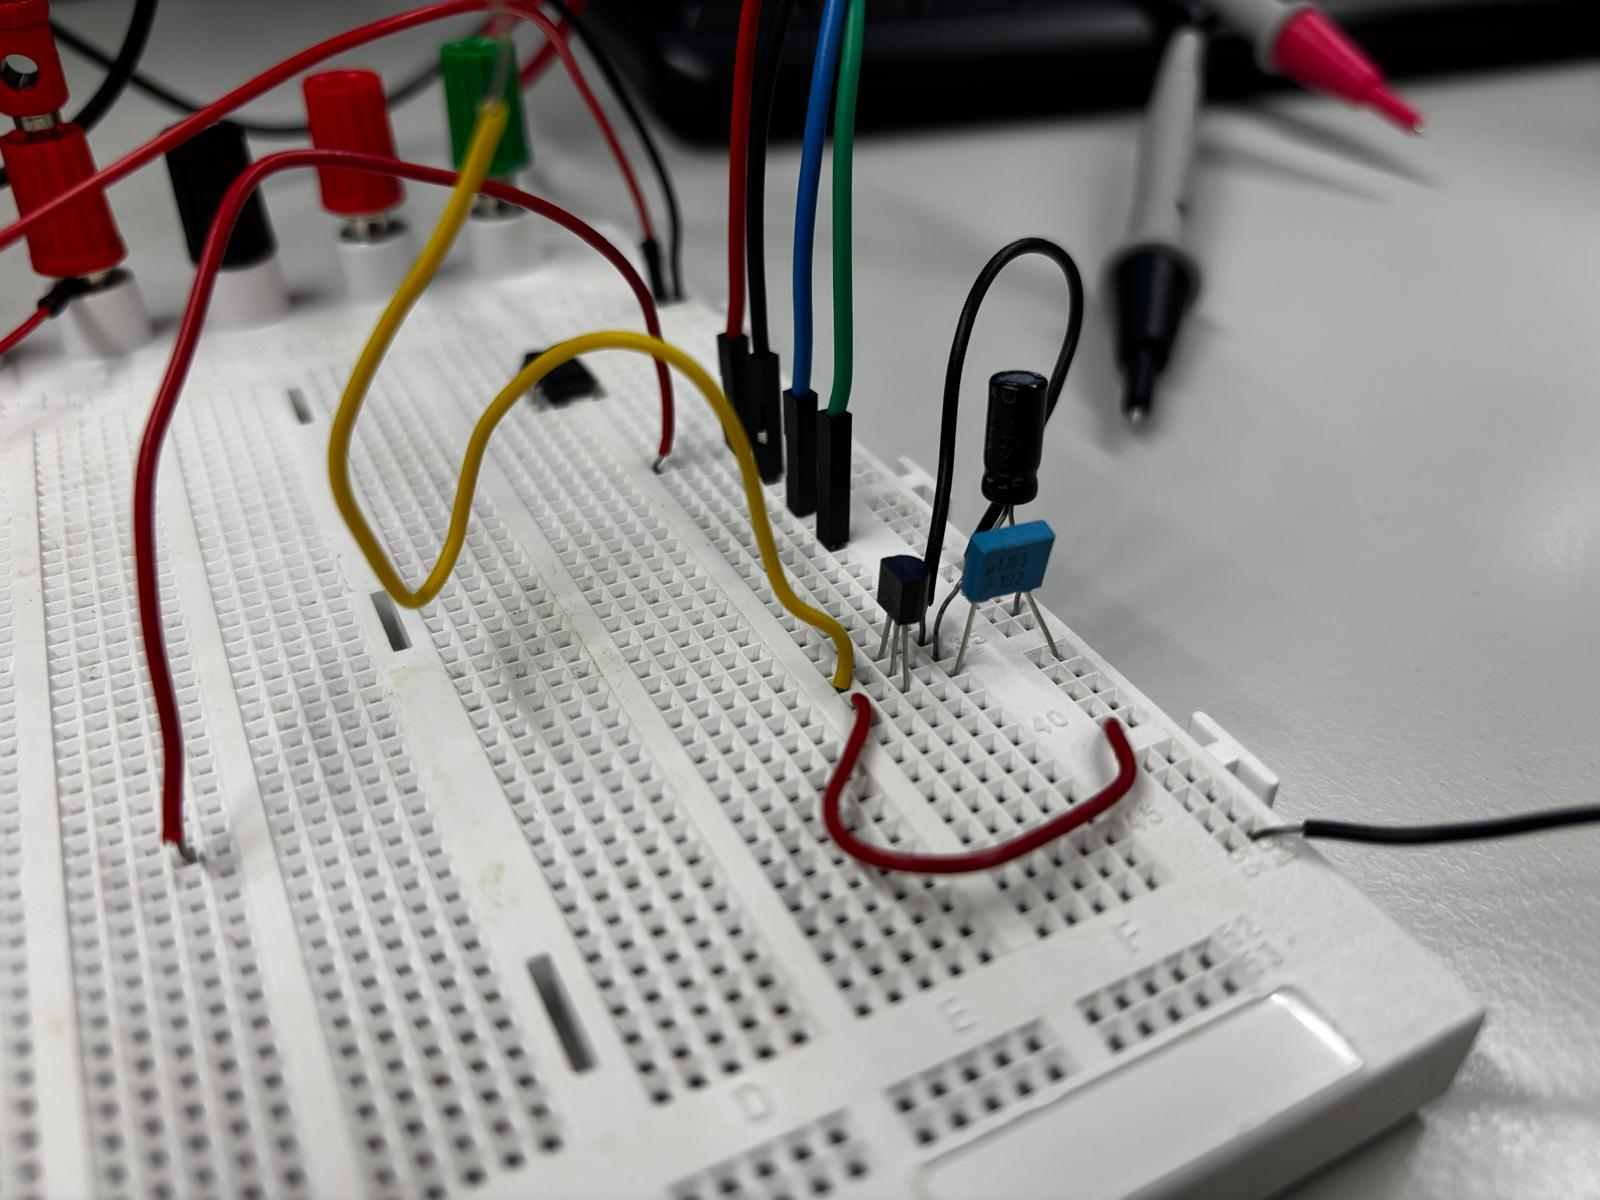
\includegraphics[width=\textwidth]{figs/vref_implementation.jpeg}
        \caption{Montaje en la \textit{protoboard}.}
        \label{fig:vref_impl}
    \end{subfigure}
    \caption{Circuito de generación de \texttt{VREF} mediante la referencia MCP1541.}
    \label{fig:vref}
\end{figure}

El valor medido experimentalmente es $V_{\mathrm{REF}} = \SI{4.1}{\V}$, lo que representa una desviación del \SI{0.097}{\percent} respecto al nominal \cite{microchip_mcp1525_2012}, dentro de la tolerancia especificada por el fabricante.

\subsection{Generación del pedestal de referencia}

Sin un nivel de referencia en el pin REF del AD623, cualquier desequilibrio de polaridad negativa en el puente empujaría la salida del amplificador hacia \SI{0}{\V}, provocando saturación. Para evitarlo, se inyecta un pedestal en el pin~5 (REF) del AD623 mediante un divisor resistivo aislado por un seguidor de tensión basado en el MCP6021 \cite{mcp6021_datasheet}.

\subsubsection*{Diseño inicial: $R_2 = \SI{22}{\kohm}$}

En una primera iteración, el divisor se dimensiona con $R_1 = \SI{68}{\kohm}$ y $R_2 = \SI{22}{\kohm}$, obteniendo un pedestal teórico de:

\[
    V_{\mathrm{PED,1}} = \SI{4.096}{\V} \cdot
    \frac{\SI{22}{\kohm}}{\SI{68}{\kohm} + \SI{22}{\kohm}}
    \approx \SI{1.0}{\V}
\]

El valor medido experimentalmente fue $V_{\mathrm{PED,1,med}} = \SI{0.9945}{\V}$, dentro de la
tolerancia esperada. Sin embargo, con este pedestal la tensión de salida del sistema con la botella de \SI{1}{\kg} resultó ser $V_{o,\mathrm{botella,1}} = \SI{2.20}{\V}$, lo que dejaba
un margen de excursión reducido hacia la plena escala (\SI{1.5}{\kg}) y comprometía la resolución efectiva del sistema.

\subsubsection*{Ajuste final: $R_2 = \SI{44}{\kohm}$}

Para aumentar la excursión de la señal de salida y mejorar la resolución, se añadió una resistencia adicional de \SI{22}{\kohm} en serie con $R_2$, elevando el pedestal a:

\[
    V_{\mathrm{PED,2}} = \SI{4.096}{\V} \cdot
    \frac{\SI{44}{\kohm}}{\SI{68}{\kohm} + \SI{44}{\kohm}}
    \approx \SI{1609.14}{\mV}
\]

Con este nuevo pedestal, la tensión de salida con la botella de \SI{1}{\kg} pasó a ser $V_{o,\mathrm{botella,2}} = \SI{2.819}{\V}$, lo que representa un incremento de \SI{0.619}{\V} respecto a la configuración anterior y amplía el rango dinámico aprovechable de la señal. El valor medido del pedestal fue $V_{\mathrm{PED,2,med}} = \SI{1.597}{\V}$, con una desviación de \SI{0.754}{\percent} respecto al valor teórico, atribuible a las tolerancias del 5\,\% de las resistencias.

Aunque el valor final del pedestal difiere del valor de \SI{1.0}{\V} nominal indicado en el enunciado, sigue cumpliendo el objetivo fundamental de mantener la salida del AD623 alejada de la saturación de masa en el peor escenario de desequilibrio del puente, garantizando además un mayor aprovechamiento del rango de entrada de la tarjeta DAQ.

\begin{figure}[H]
    \centering
    %\includesvg[width=0.65\textwidth]{figs/CKTO MCP6021}
    \caption{Circuito generador del pedestal de referencia
        en su configuración final: divisor resistivo
        ($R_1 = \SI{68}{\kohm}$,
        $R_2 = 2 \times \SI{22}{\kohm} = \SI{44}{\kohm}$)
        y seguidor MCP6021 con salida al pin~5 (REF)
        del AD623.}
    \label{fig:pedestal}
\end{figure}


\subsection{Análisis de Tolerancias (Worst-Case DC)}

En esta sección se presenta la tensión de error máxima prevista a la salida del sistema de acondicionamiento bajo condiciones de reposo (sin carga aplicada). Se implementó el modelo de análisis para el peor escenario, este modelo asume la superposición lineal de todas las fuentes de error del sensor y de la etapa de amplificación, alineadas en la polaridad más desfavorable para inducir la máxima desviación posible antes de la saturación del sistema.

\subsubsection{Cálculo del error inherente del sensor}

El primer término de error proviene del desequilibrio físico del puente de Wheatstone. Se estableció un desequilibrio sin carga equivalente al 5\% de la salida a fondo de escala (FSO). Considerando la tensión de excitación unipolar de 4.096 voltios (proporcionado por la referencia del MCP1541) y la sensibilidad nominal de la célula de carga de 1 $\text{mV/V}$, la salida a fondo de escala se define como:

$$V_{FSO}=V_{EXC} \cdot \text{Sensibilidad} = 4.096 \text{V} \cdot 1 \text{ mV/V} = 4.096 \text{ mV}$$

Por lo que la tensión de error diferencial intrínseca aportada por el sensor en reposo es:

$$V_{err\_sensor}=0.05 \cdot V_{FSO} = 0.05 \cdot 4.096 \text{ mV} = 0.2048 \text{ mV}$$

\subsubsection{Error de la etapa de amplificación}

La segunda etapa de error derivó del amplificador de instrumentación AD623. En el diseño implementado, la ganancia (G) se fijó mediante una resistencia $R_{G} = 50.2 \text{ }\Omega $. Aplicando la ecuación de la ganancia del fabricante \cite{ad623_datasheet}:

$$\text{GAIN} = 1+100\text{ k}\Omega/R_G = 1+100\text{ k}\Omega/50.2\text{ }\Omega$$
$$\text{GAIN} = 1993.032 \text{ V/V} $$

\subsubsection{Errores referidos a la entrada (amplificados por la ganancia G)}

\begin{itemize}
    \item Tensión de offset de entrada ($V_{OSI}$): De acuerdo con las especificaciones del fabricante \cite{ad623_datasheet}, el valor máximo es de 200 $\mu$ \unit{V} = 0.2 m\unit{V}
    \item Caída de tensión por la corriente de offset ($V_{err\_IB}$): En el esquema de diseño, las entradas del AD623 están precedidas por un filtro pasivo contra interferencias de radiofrecuencia (RFI) compuesto por las resistencias R1 = R2 = 15.9 k $\Omega$. Al circilar la corriente de offset de entrada ($I_{OS}$) (de acuerdo con \cite{ad623_datasheet}, es de 2 \text{ nA}), a través de estas resistencias, se induce un error diferencial adicional evaluado en:
          $$V_{err\_IB} = I_{OS} \cdot R_{filtro} = 2 \text{ nA} \cdot 15.9 \text{ k} \Omega=  0.0318 \text{ mV}$$
\end{itemize}

\subsubsection{Errores referidos a la salida (independientes de la ganancia)}

\begin{itemize}
    \item Tensión de offset de salida ($V_{OSO}$): El fabricante especifica un valor máximo de 1000 $\mu$V = 1 m\unit{V}.
\end{itemize}

\subsubsection{Ecuación global del peor escenario y contraste de saturación}

Aplicando el factor de amplificación de la etapa (G = 1993.032 V/V), solo a las perturbaciones generadas a la entrada del sistema, la ecuación analítica del error máximo en corriente continua es:

$$V_{error\_MAX}=G \cdot (V_{err\_sensor} + V_{OSI} + V_{err\_IB}) + V_{OSO}$$

$$V_{error\_MAX}= 1993.032 \cdot (0.2048 \text{ mV} + 0.2 \text{ mV} + 0.0318 \text{ mV}) + 1 \text
    { mV}$$

$$V_{error\_MAX}= 871.16 \text
    { mV}$$

Para determinar la tensión estática absoluta en el terminal de salida del acondicionador ($V_{OUT\_reposo}$), se debe superponer el voltaje del pedestal virtual de 1609.14 m\unit{V}, introducido en el terminal de referencia (REF) del AD623 mediante la etapa aislada del amplificador operacional MCP6021.

$$ V_{OUT\_reposo} = V_{pedestal} \pm V_{error\_MAX} = 1609.14 \text{ mV} \pm 871.16 \text{ mV} $$

$$ V_{OUT\_reposo} = \{737.98 \text{ - } 2480.3\} \text{ mV}$$

De acuerdo con el resultado anterior, se puede constatar que el nivel de tensión en reposo se mantiene dentro del rango de trabajo de la entrada analógica de la tarjeta DAQ NI USB-6001.

\section{Acondicionamiento Dinámico (Filtrado AC y Adquisición)}
\subsection{Filtro RFI de entrada}

Las señales $V_a$ y $V_b$ procedentes de la célula de carga pasan cada una por un filtro paso bajo de primer orden antes de entrar a los pines IN+ (pin~3) e IN$-$ (pin~2) del AD623. Cada rama incorpora una resistencia $R_w = \SI{15.9}{\kohm}$ y un condensador de \SI{100}{\nano\F} a masa (dieléctrico de poliéster), con una frecuencia de corte de modo común de:
\[
    f_{c,\mathrm{CM}} = \frac{1}{2\pi \cdot R_w \cdot C}
    = \frac{1}{2\pi \times \SI{15.9}{\kohm}
        \times \SI{100}{\nano\F}}
    \approx \SI{100}{\Hz}
\]
Adicionalmente, se conecta un condensador diferencial de \SI{1}{\micro\F} directamente entre los pines~2 y~3 del AD623, cuya frecuencia de corte diferencial es:
\[
    f_{c,\mathrm{dif}} = \frac{1}{2\pi \cdot 2R_w \cdot C_{\mathrm{dif}}}
    = \frac{1}{2\pi \times \SI{31.8}{\kohm}
        \times \SI{1}{\micro\F}}
    \approx \SI{5.0}{\Hz}
\]
Este condensador diferencial reduce el ruido de modo diferencial de alta frecuencia, complementando la atenuación de modo común del filtro de entrada. El uso de condensadores de película de poliéster en ambas ramas es un requisito crítico de diseño: su tolerancia ajustada garantiza el equilibrio de impedancias entre las dos ramas y preserva el CMRR del AD623 \cite{ad623_datasheet}. Un desequilibrio entre los condensadores degradaría directamente la capacidad del amplificador de rechazar el ruido de modo común.

\begin{figure}[H]
    \centering
    %\includesvg[width=0.70\textwidth]{figs/CKTO AD623}
    \caption{Filtro RFI de entrada: resistencias $R_w$ y condensadores
        a masa en cada rama, y condensador diferencial de
        \SI{1}{\micro\F} entre los pines de entrada del AD623.}
    \label{fig:filtro_rfi}
\end{figure}

\subsection{Red de adaptación de salida}

La salida del AD623 y la tensión de referencia del pedestal no se conectan directamente a masa en la tarjeta DAQ, sino que se adquieren como dos canales independientes (AI0 y AI4) y su diferencia se calcula por \textit{software} en \textit{LabVIEW}. Esta topología permite rechazar la deriva térmica del pedestal, que afecta por igual a ambas señales y queda cancelada al restarlas \cite{ni6001_datasheet}. Para garantizar el equilibrio de impedancias entre ambas líneas, cada una pasa por un filtro RC simétrico antes de entrar a la DAQ:
\begin{itemize}
    \item $V_o$ (salida AD623) → $R_f = \SI{13.7}{\kohm}$, $C_f = \SI{2.2}{\micro\F}$ → AI0, con $f_c \approx \SI{5.28}{\Hz}$
    \item $V_{\mathrm{REF}}$ (pedestal) → $R = \SI{13.7}{\kohm}$, $C = \SI{2.2}{\micro\F}$ → AI4, con $f_c \approx \SI{5.28}{\Hz}$
\end{itemize}
El equilibrio de estas impedancias es esencial: cualquier asimetría introduciría una diferencia de fase entre ambas señales que la resta por \textit{software} no podría compensar, degradando el rechazo a la deriva del pedestal \cite{ni6001_datasheet}.

\begin{figure}[H]
    \centering
    %\includesvg[width=0.70\textwidth]{figs/CKTO FILTRO}
    \caption{Red de adaptación de salida: filtros RC simétricos
        en las líneas $V_o$ y $V_{\mathrm{REF}}$ hacia los
        canales AI0 y AI4 de la NI USB-6001.}
    \label{fig:filtro_salida}
\end{figure}

\section{Análisis de Ruido y Cuantización}
\subsection{Balance de error dinámico (límite analógico)}

MMmmm
El límite físico de detección del sistema está determinado por el ruido intrínseco del hardware, compuesto fundamentalmente por el ruido térmico de las resistencias y el ruido del amplificador de instrumentación.


\section{Diseño del Instrumento Virtual (LabVIEW)}
En la figura \ref{fig:diagrama_bloques}, se muestra el diagrama de bloques general desarrollado en \textit{LabVIEW}.

\begin{figure}[H]
    \centering
    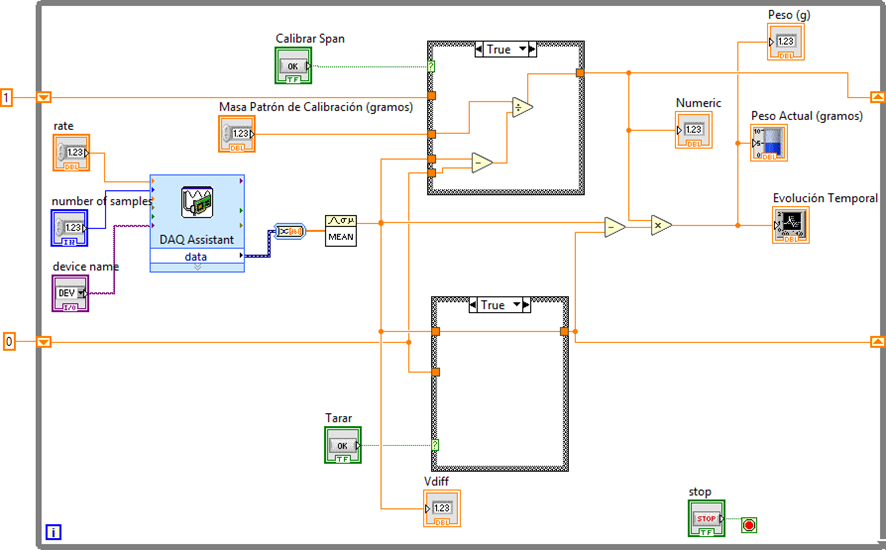
\includegraphics[width=1\linewidth]{figs/diagrama_bloques_LABVIEW.png}
    \caption{Diagrama de Bloques general en \textit{LabVIEW}.}
    \label{fig:diagrama_bloques}
\end{figure}

La ejecución del programa está encapsulada dentro de un bucle \textit{While}, lo que permite la iteración ininterrumpida del proceso de lectura, cálculo y visualización hasta que el operador detenga el sistema de manera manual mediante el control de parada incorporado en la interfaz.


\subsection{Adquisición y Acondicionamiento de la Señal}

Se utilizó el bloque \textit{DAQ Assistant}, el cual está configurado para interrogar al hardware físico. Se seleccionó un terminal de entrada en modo diferencial frente a la configuración RSE (Referenciado a Masa), tal como se ilustra en la figura \ref{fig:diferencial}. Esta decisión de diseño es imperativa para preservar el factor de rechazo al modo común (CMRR) de la etapa de acondicionamiento analógico previa, mitigando el ruido eléctrico en modo común inducido en las líneas de transmisión de la señal de bajo nivel proveniente de la célula de carga.

\begin{figure}[H]
    \centering
    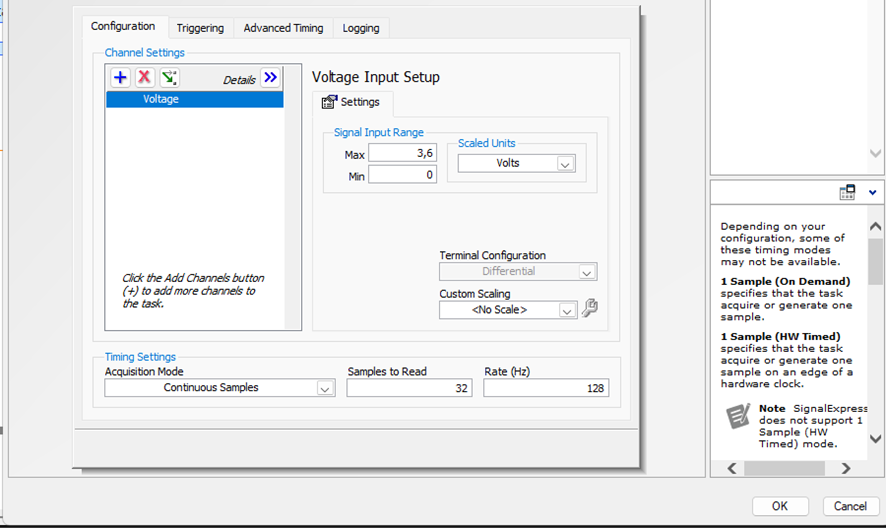
\includegraphics[width=0.75\linewidth]{figs/diferencial.png}
    \caption{Configuración en Modo diferencial en el módulo \textit{DAQ Assistant}.}
    \label{fig:diferencial}
\end{figure}

Este bloque adquiere la señal de tensión analógica, parametrizando un rango de tensión de $\pm3.6$ V] para maximizar la resolución del convertidor. La lectura de la información se realiza en paquetes definidos por una frecuencia de muestreo (\textit{Rate}) de 128 Hz y un número de muestras (\textit{Samples to Read}) establecido en exactamente 32 muestras.

Esta ventana de promediado estadístico por software se justifica como el punto de operación óptimo del instrumento virtual: un número inferior de muestras resultaría en un filtrado insuficiente del ruido térmico y de cuantización, provocando inestabilidad en el dígito menos significativo de la lectura física; por el contrario, una ventana mayor introduciría una latencia considerable en el bucle, degradando el tiempo de respuesta dinámico de la báscula frente a variaciones súbitas de carga. Los datos dinámicos obtenidos en esta ventana pasan de forma directa por un bloque estadístico de media aritmética (\textit{Mean}), entregando un único valor de tensión estabilizado para las etapas posteriores de procesamiento matemático.

\subsection{Arquitectura del VI y Gestión de Memoria Dinámica}

Para mantener las constantes de calibración actualizadas y disponibles ciclo tras ciclo, el diagrama de bloques emplea dos registros de desplazamiento (\textit{Shift Registers}) ubicados en los bordes laterales del bucle \textit{While} principal:

\begin{itemize}
    \item \textbf{Registro Superior (Factor de \textit{Span}):} Inicializado con una constante de valor 1, almacena el multiplicador dinámico que convierte la magnitud eléctrica neta a unidades físicas de masa (gramos).
    \item \textbf{Registro Inferior (Tensión de Tara):} Inicializado en 0 V, retiene el valor de la tensión residual medida sin carga, el cual se corresponde con el cero del sistema.
\end{itemize}

En la figura \ref{fig:estructuras_case} se detalla la lógica interna de almacenamiento según los estados de control del operador.

\begin{figure}[H]
    \centering
    \begin{subfigure}[b]{0.48\textwidth}
        \centering
        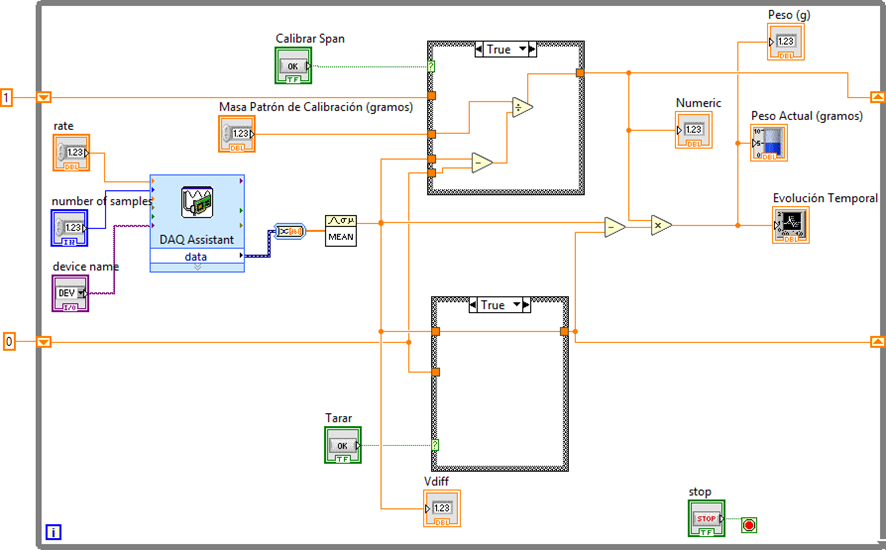
\includegraphics[width=\textwidth]{figs/diagrama_bloques_LABVIEW.png}
        \caption{Diagrama de bloques (Caso \textit{True}).}
        \label{fig:labview_caso_true}
    \end{subfigure}
    \hfill
    \begin{subfigure}[b]{0.48\textwidth}
        \centering
        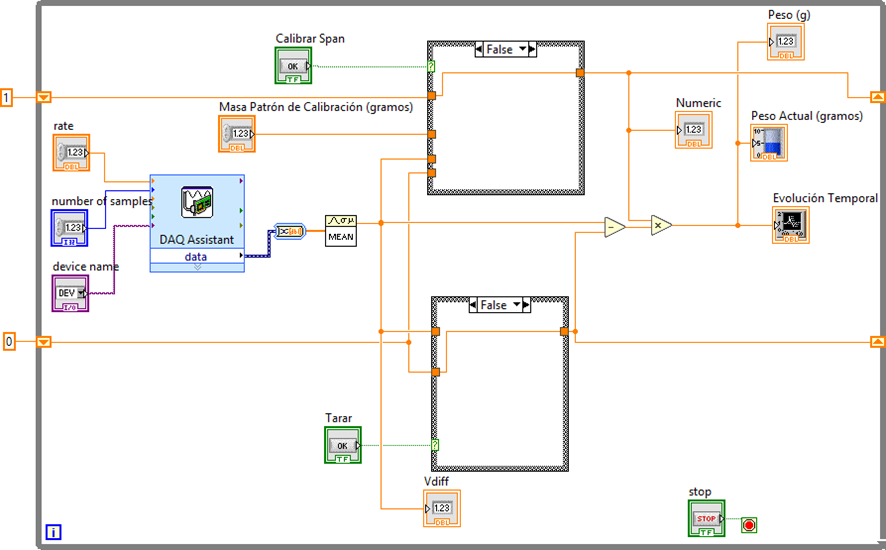
\includegraphics[width=\textwidth]{figs/labview_caso_false.png}
        \caption{Diagrama de bloques (Caso \textit{False}).}
        \label{fig:labview_caso_false}
    \end{subfigure}
    \caption{Comportamiento de la arquitectura interna del VI según los eventos de control.}
    \label{fig:estructuras_case}
\end{figure}

\subsection{Lógica Matemática y Rutinas Condicionales de Calibración}

El software cuenta con un algoritmo de calibración lineal de dos puntos gestionado por estructuras \textit{Case}. Estas rutinas son accionadas a voluntad por el usuario a través del Panel Frontal:

\begin{itemize}
    \item \textbf{Establecimiento del Cero (Tara):} Controlado por la estructura inferior (ver figura \ref{fig:establecer_cero_labview}). Al recibir un comando lógico verdadero (\textit{True}) tras pulsar el botón de tara, el programa captura la tensión promedio instantánea de ese ciclo exacto y la sobrescribe en el \textit{Shift Register} inferior. En su estado inactivo (\textit{False}), el último valor registrado simplemente atraviesa la estructura para mantenerse intacto en la memoria dinámica.
    \item \textbf{Calibración del \textit{Span}:} Controlada por la estructura superior (ver figura \ref{fig:establecer_span}). Al introducir el valor de la masa patrón en la interfaz y activar esta rutina, el programa recalcula la pendiente de medición. Obtiene la tensión neta bajo carga y ejecuta la siguiente relación matemática:

          $$Factor=\frac{\text{Masa}_{\text{referencia}}}{V_{leido}-V_{tara}}$$

          El resultado numérico de esta operación sobrescribe el registro de desplazamiento superior, actualizando la sensibilidad global del instrumento de manera instantánea.
\end{itemize}

\begin{figure}[H]
    \centering
    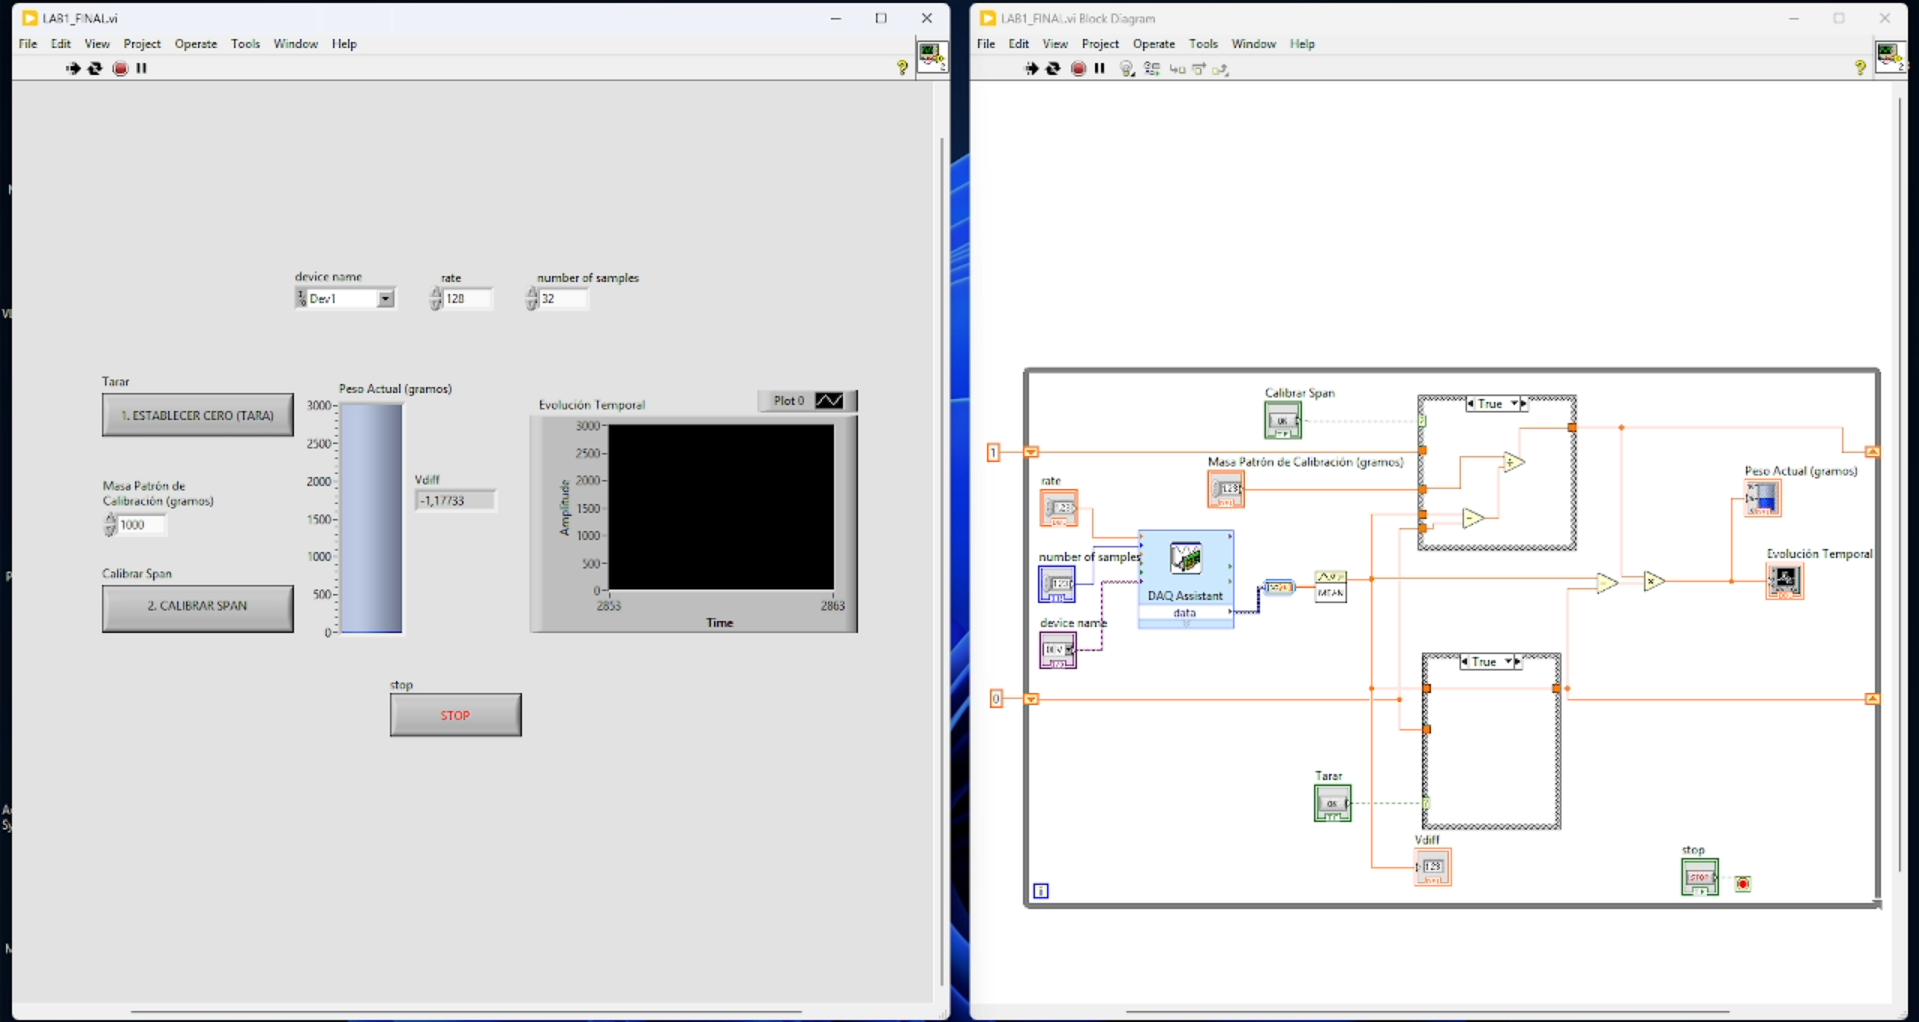
\includegraphics[width=1\linewidth]{figs/establecer_cero_labview.png}
    \caption{Diagrama de bloques ante la activación del evento de Establecer Cero.}
    \label{fig:establecer_cero_labview}
\end{figure}

\begin{figure}[H]
    \centering
    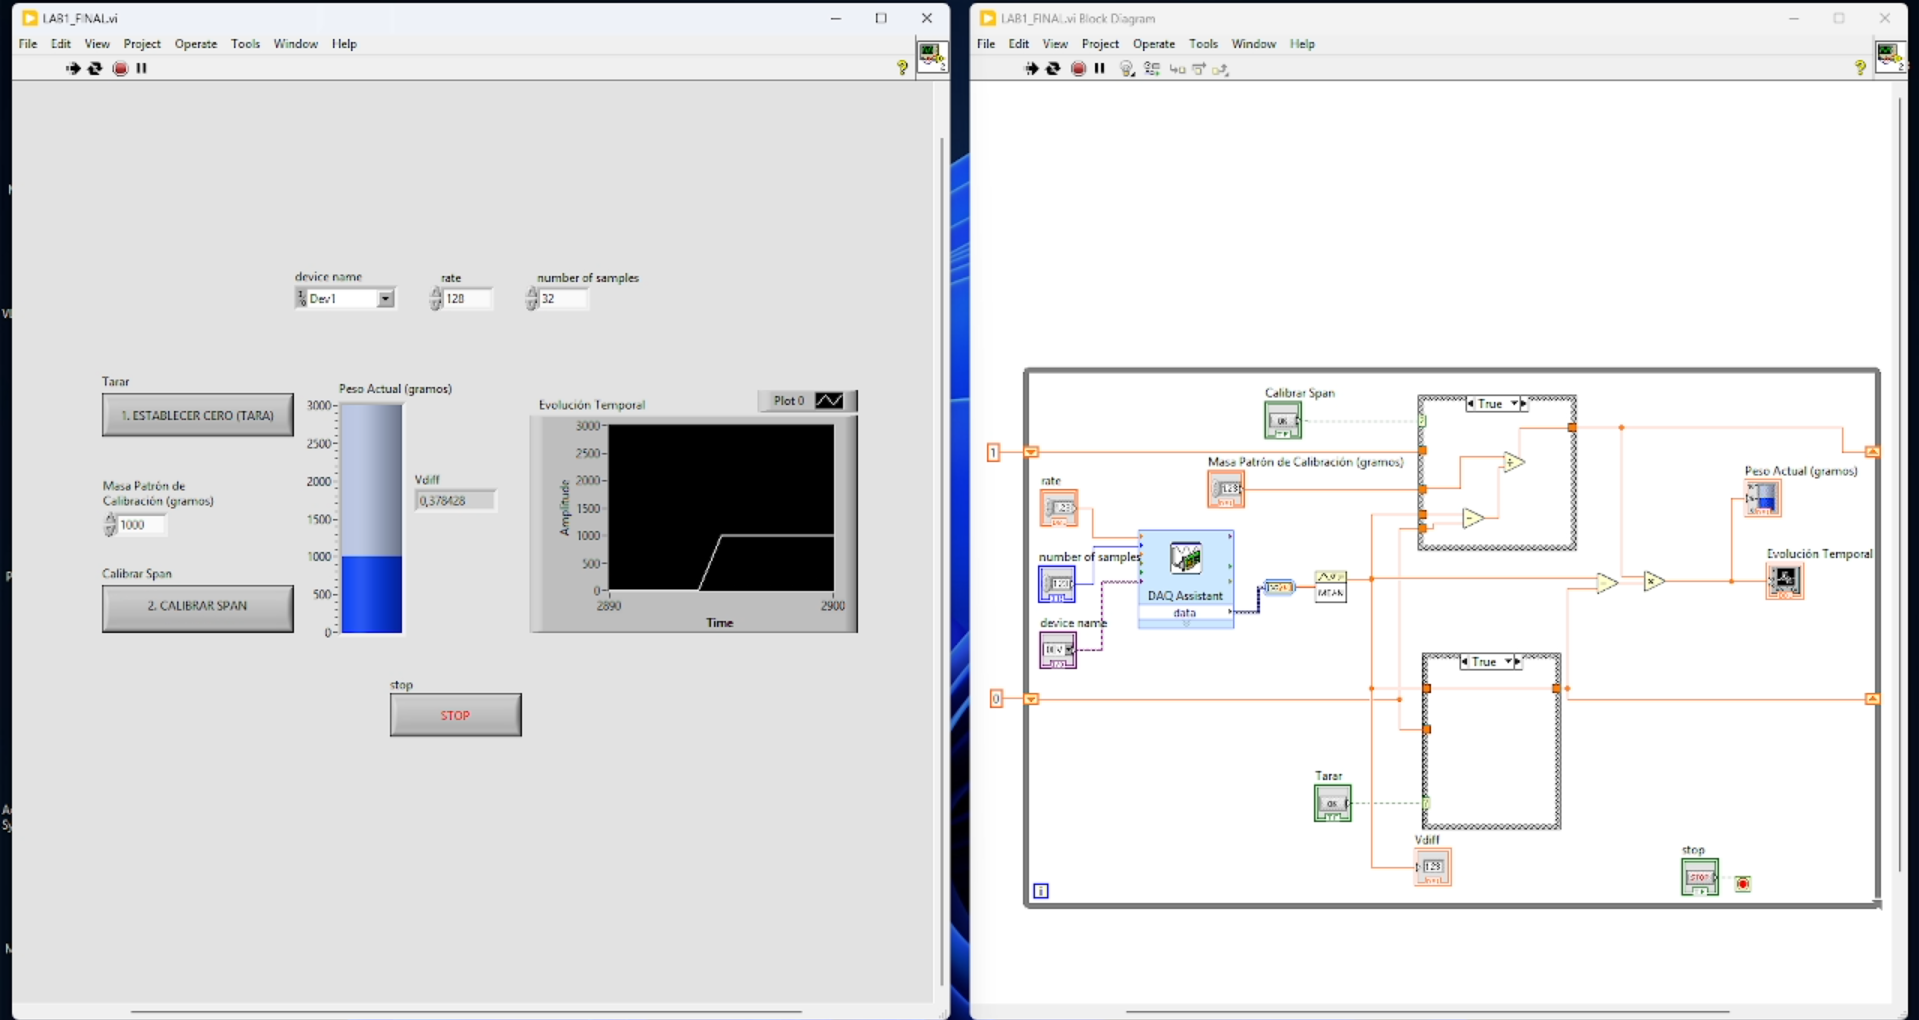
\includegraphics[width=1\linewidth]{figs/establecer_span.png}
    \caption{Diagrama de bloques ante la activación del ajuste de \textit{Span} utilizando la masa patrón de 1.000 kg.}
    \label{fig:establecer_span}
\end{figure}

\subsection{Procesamiento Final, Monitorización e Interfaz de Usuario}

De forma paralela a las lógicas condicionales, el diagrama ejecuta en cada iteración el cálculo lineal definitivo para obtener la masa real. Utilizando nodos aritméticos elementales, se aplica la ecuación de la recta basada en las señales en tiempo real y las constantes retenidas en la memoria dinámica:

$$Peso=(V_{leido}-V_{tara}) \times Factor$$

El resultado numérico representa la magnitud calibrada final. A nivel de Panel Frontal, la interfaz ha sido diseñada bajo criterios ergonómicos, priorizando la legibilidad metrológica de los indicadores. La magnitud calculada alimenta simultáneamente tres elementos gráficos visualmente jerarquizados: un indicador numérico de gran tamaño para la lectura directa rápida, un indicador de barra vertical para evaluar el rango dinámico consumido respecto al fondo de escala (\textit{FSO}), y un gráfico de tipo \textit{Waveform Chart}. Este último elemento gráfico es vital desde la perspectiva metrológica, pues permite al operador monitorizar visualmente la estabilidad temporal del puente, evaluar el tiempo de asentamiento de la señal tras depositar una masa y verificar la correcta mitigación del ruido analógico por el software.

En las figuras \ref{fig:pesajecero} y \ref{fig:pesajedeprueba} se muestra el comportamiento operativo de la interfaz en sus dos estados fundamentales de carga.

\begin{figure}[H]
    \centering
    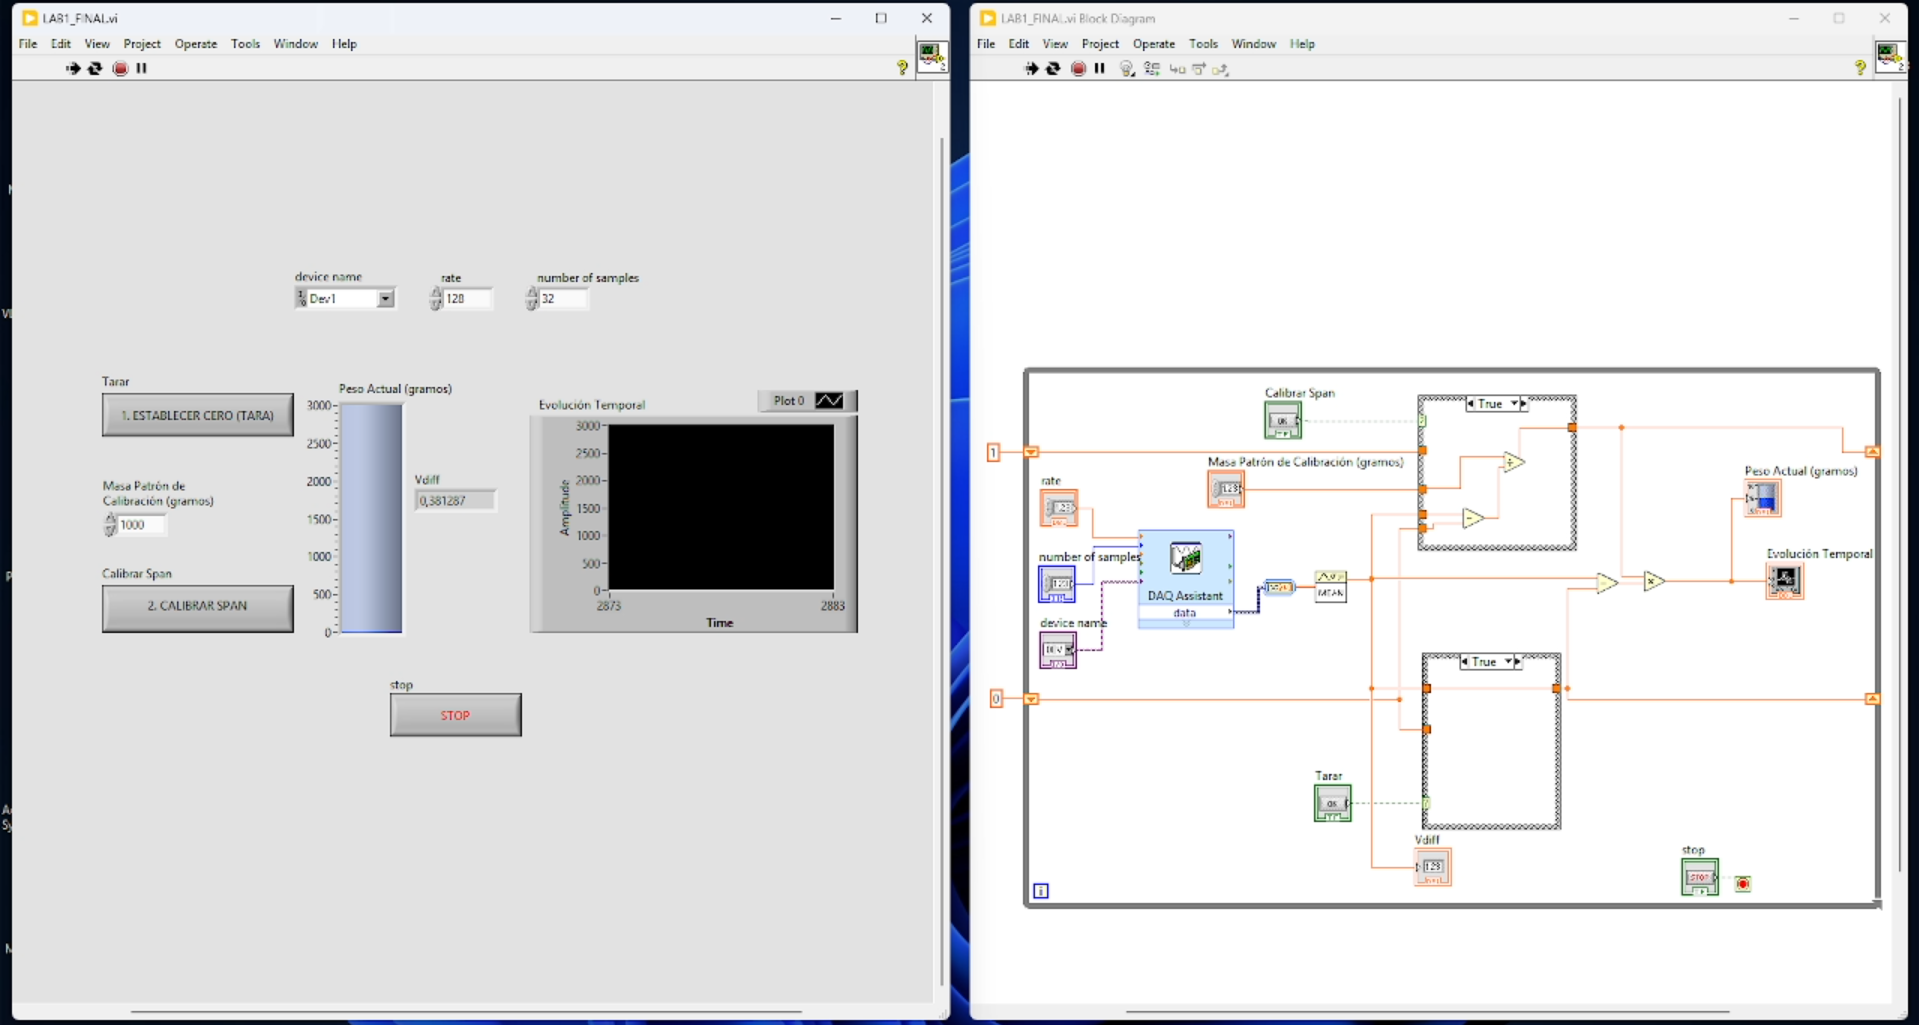
\includegraphics[width=1\linewidth]{figs/pesajecero.png}
    \caption{Interfaz del Panel Frontal en estado de reposo (Fijación del cero metrológico).}
    \label{fig:pesajecero}
\end{figure}

\begin{figure}[H]
    \centering
    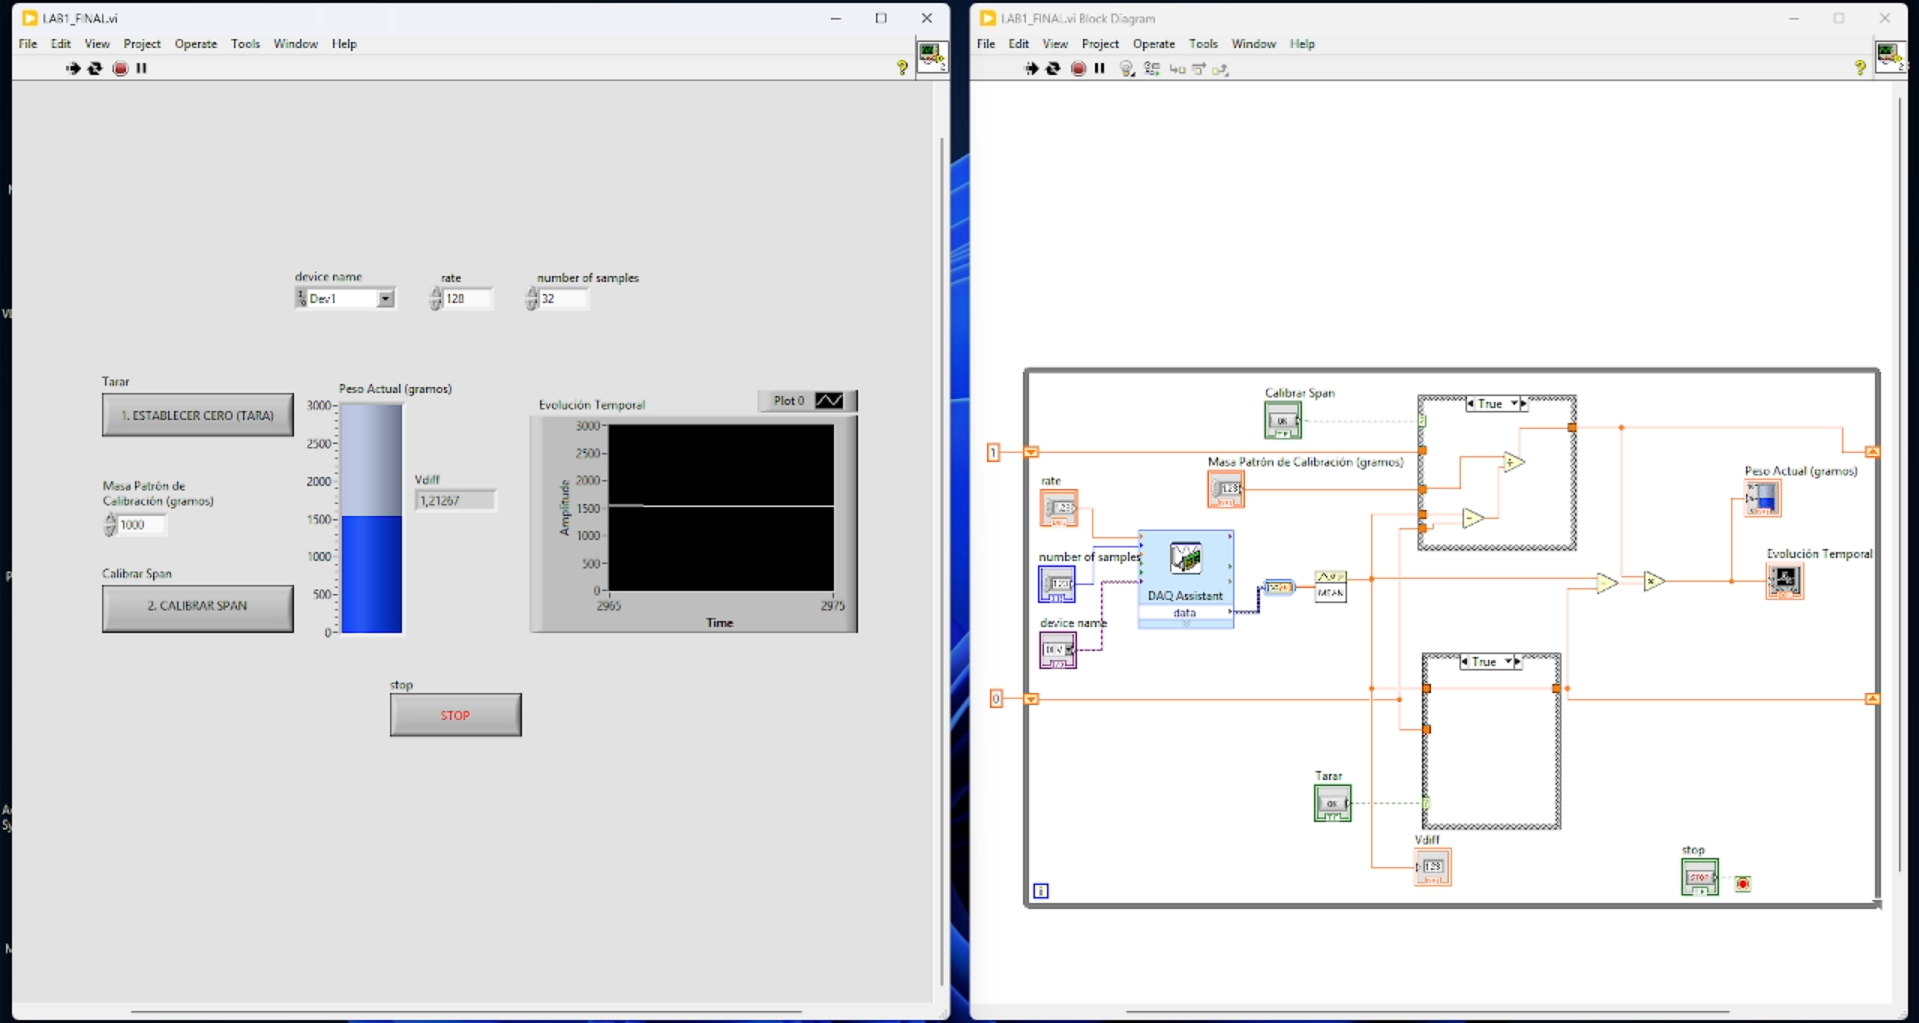
\includegraphics[width=1\linewidth]{figs/pesajedeprueba.png}
    \caption{Validación experimental del sistema mediante el pesaje de una masa de prueba de 1.5 kg.}
    \label{fig:pesajedeprueba}
\end{figure}

\section{Validación y Resultados Experimentales}
\subsection{Metodología de Calibración}

El ajuste del instrumento virtual se llevó a cabo mediante un procedimiento de calibración lineal de dos puntos. Este proceso permitió corregir los errores sistemáticos de la etapa de acondicionamiento analógico y establecer la trazabilidad de las medidas.

\begin{enumerate}
    \item \textbf{Fijación del Cero Metrológico (\textit{Tara}):} Con el sistema mecánico en reposo y la plataforma de pesaje completamente vacía, se procedió a la captura de la tensión residual. Esta medición en crudo absorbe el desequilibrio estático del puente de Wheatstone, las tensiones de \textit{offset} del amplificador de instrumentación AD623 y el pedestal de referencia de 1.607~voltios. El algoritmo en \textit{LabVIEW} almacena este valor como el cero del sistema, restándolo de forma sistemática en las lecturas subsecuentes.
    
    \item \textbf{Ajuste del \textit{Span} (Pendiente):} Posteriormente, se aplicó sobre la célula de carga una masa de referencia aproximado de 1.000~kg, empleado como peso patrón. Al estabilizarse la señal, el \textit{software} registró la tensión neta correspondiente al fondo de escala operativo y calculó de forma automática el factor de ganancia global (pendiente de la recta de calibración).
\end{enumerate}

La sensibilidad empírica resultante del proceso de calibración arrojó un valor de 642.49~\si{\frac{V}{g}}.

Este valor se calculó teóricamente de la siguiente manera, se tomaron dos medidas:

\begin{itemize}
    \item $V_{diff}$ (sin carga): -1.17588 \si{V}
    \item $V_{diff}$ (con carga de 1 \si{kg}): 0.378307 \si{V}
\end{itemize}

Hallamos la sensibilidad del sistema con esos valores: 

\begin{itemize}
    \item Sensibilidad en \si{\frac{V}{g}}
    $S=\frac{0.378307 - (-1.17588)}{1000} = 0.001554 $ \si{\frac{V}{g}}
    \item Sensibilidad en \si{\frac{g}{V}}
    $S=\frac{1000}{0.378307 - (-1.17588)} = 643.42 $ \si{\frac{g}{V}}
\end{itemize}



\subsection{Análisis de Desempeño y Caracterización Metrológica}

Para evaluar de manera crítica el comportamiento dinámico y estático del sistema, se realizó una caracterización completa que abarca el rango dinámico, la linealidad y la estabilidad temporal de la lectura.

\subsubsection{Contraste Empírico sin Carga}
Antes de la supresión por \textit{software} mediante la tara, se midió físicamente la tensión sin carga directamente a la salida del amplificador de instrumentación, registrándose un valor experimental de [COMPLETAR]~V. Este resultado se contrastó con el límite teórico de seguridad calculado en el análisis de tolerancias (\textit{Worst-Case DC}) de la sección 2. Dado que el valor experimental se encuentra notablemente por debajo del umbral de saturación previsto en el peor escenario de polaridad, se demuestra matemáticamente la validez del pedestal de referencia de 1.607~V introducido para evitar el corte en el canal de adquisición.

\subsubsection{Linealidad y Rango Dinámico}
El rango dinámico verificado de la báscula se extiende desde los 0~g hasta un límite superior de carga de 5~kg, asegurando márgenes de seguridad frente a la saturación del ADC de la tarjeta de adquisición de datos (DAQ).

El error de linealidad máximo registrado fue de [COMPLETAR]~g, confirmando un comportamiento altamente lineal en todo el rango de operación debido a la simetría simétrica de la red de filtros analógicos y al equilibrio de impedancias preservado.

\subsubsection{Estabilidad de la Lectura y Resolución Efectiva}
El impacto del promediado estadístico implementado en el instrumento virtual se demostró empíricamente al contrastar la señal en crudo frente a la señal filtrada.

Tras activar la ventana de promediado por bloques de 32 muestras en \textit{LabVIEW}, se logró una disminución  de las fluctuaciones de alta frecuencia, demostrando una mejora en la resolución efectiva del sistema sin comprometer el tiempo de respuesta demandado para el pesaje estático.

\subsection{Montaje Físico y Disposición Mecánica}

El montaje físico final se muestra en la figura \ref{fig:montaje_hardware} muestra la implementación de la etapa analógica en la placa de pruebas, caracterizada por un ruteado simétrico para proteger el CMRR. Por otro lado, la figura \ref{fig:celda_carga} ilustra la disposición mecánica de la célula de carga acoplada a la estructura rígida de soporte.

\begin{figure}[H]
    \centering
    \includegraphics[width=0.8\linewidth]{figs/montaje_hardware.png}
    \caption{Montaje físico real de la etapa de acondicionamiento eléctrico en la placa de pruebas.}
    \label{fig:montaje_hardware}
\end{figure}


\begin{figure}[H]
    \centering
    \includegraphics[width=0.8\linewidth]{figs/celda_carga.png}
    \caption{Disposición mecánica de la célula de carga y su acoplamiento estructural para el pesaje.}
    \label{fig:celda_carga}
\end{figure}



\begin{figure}[H]
    \centering
    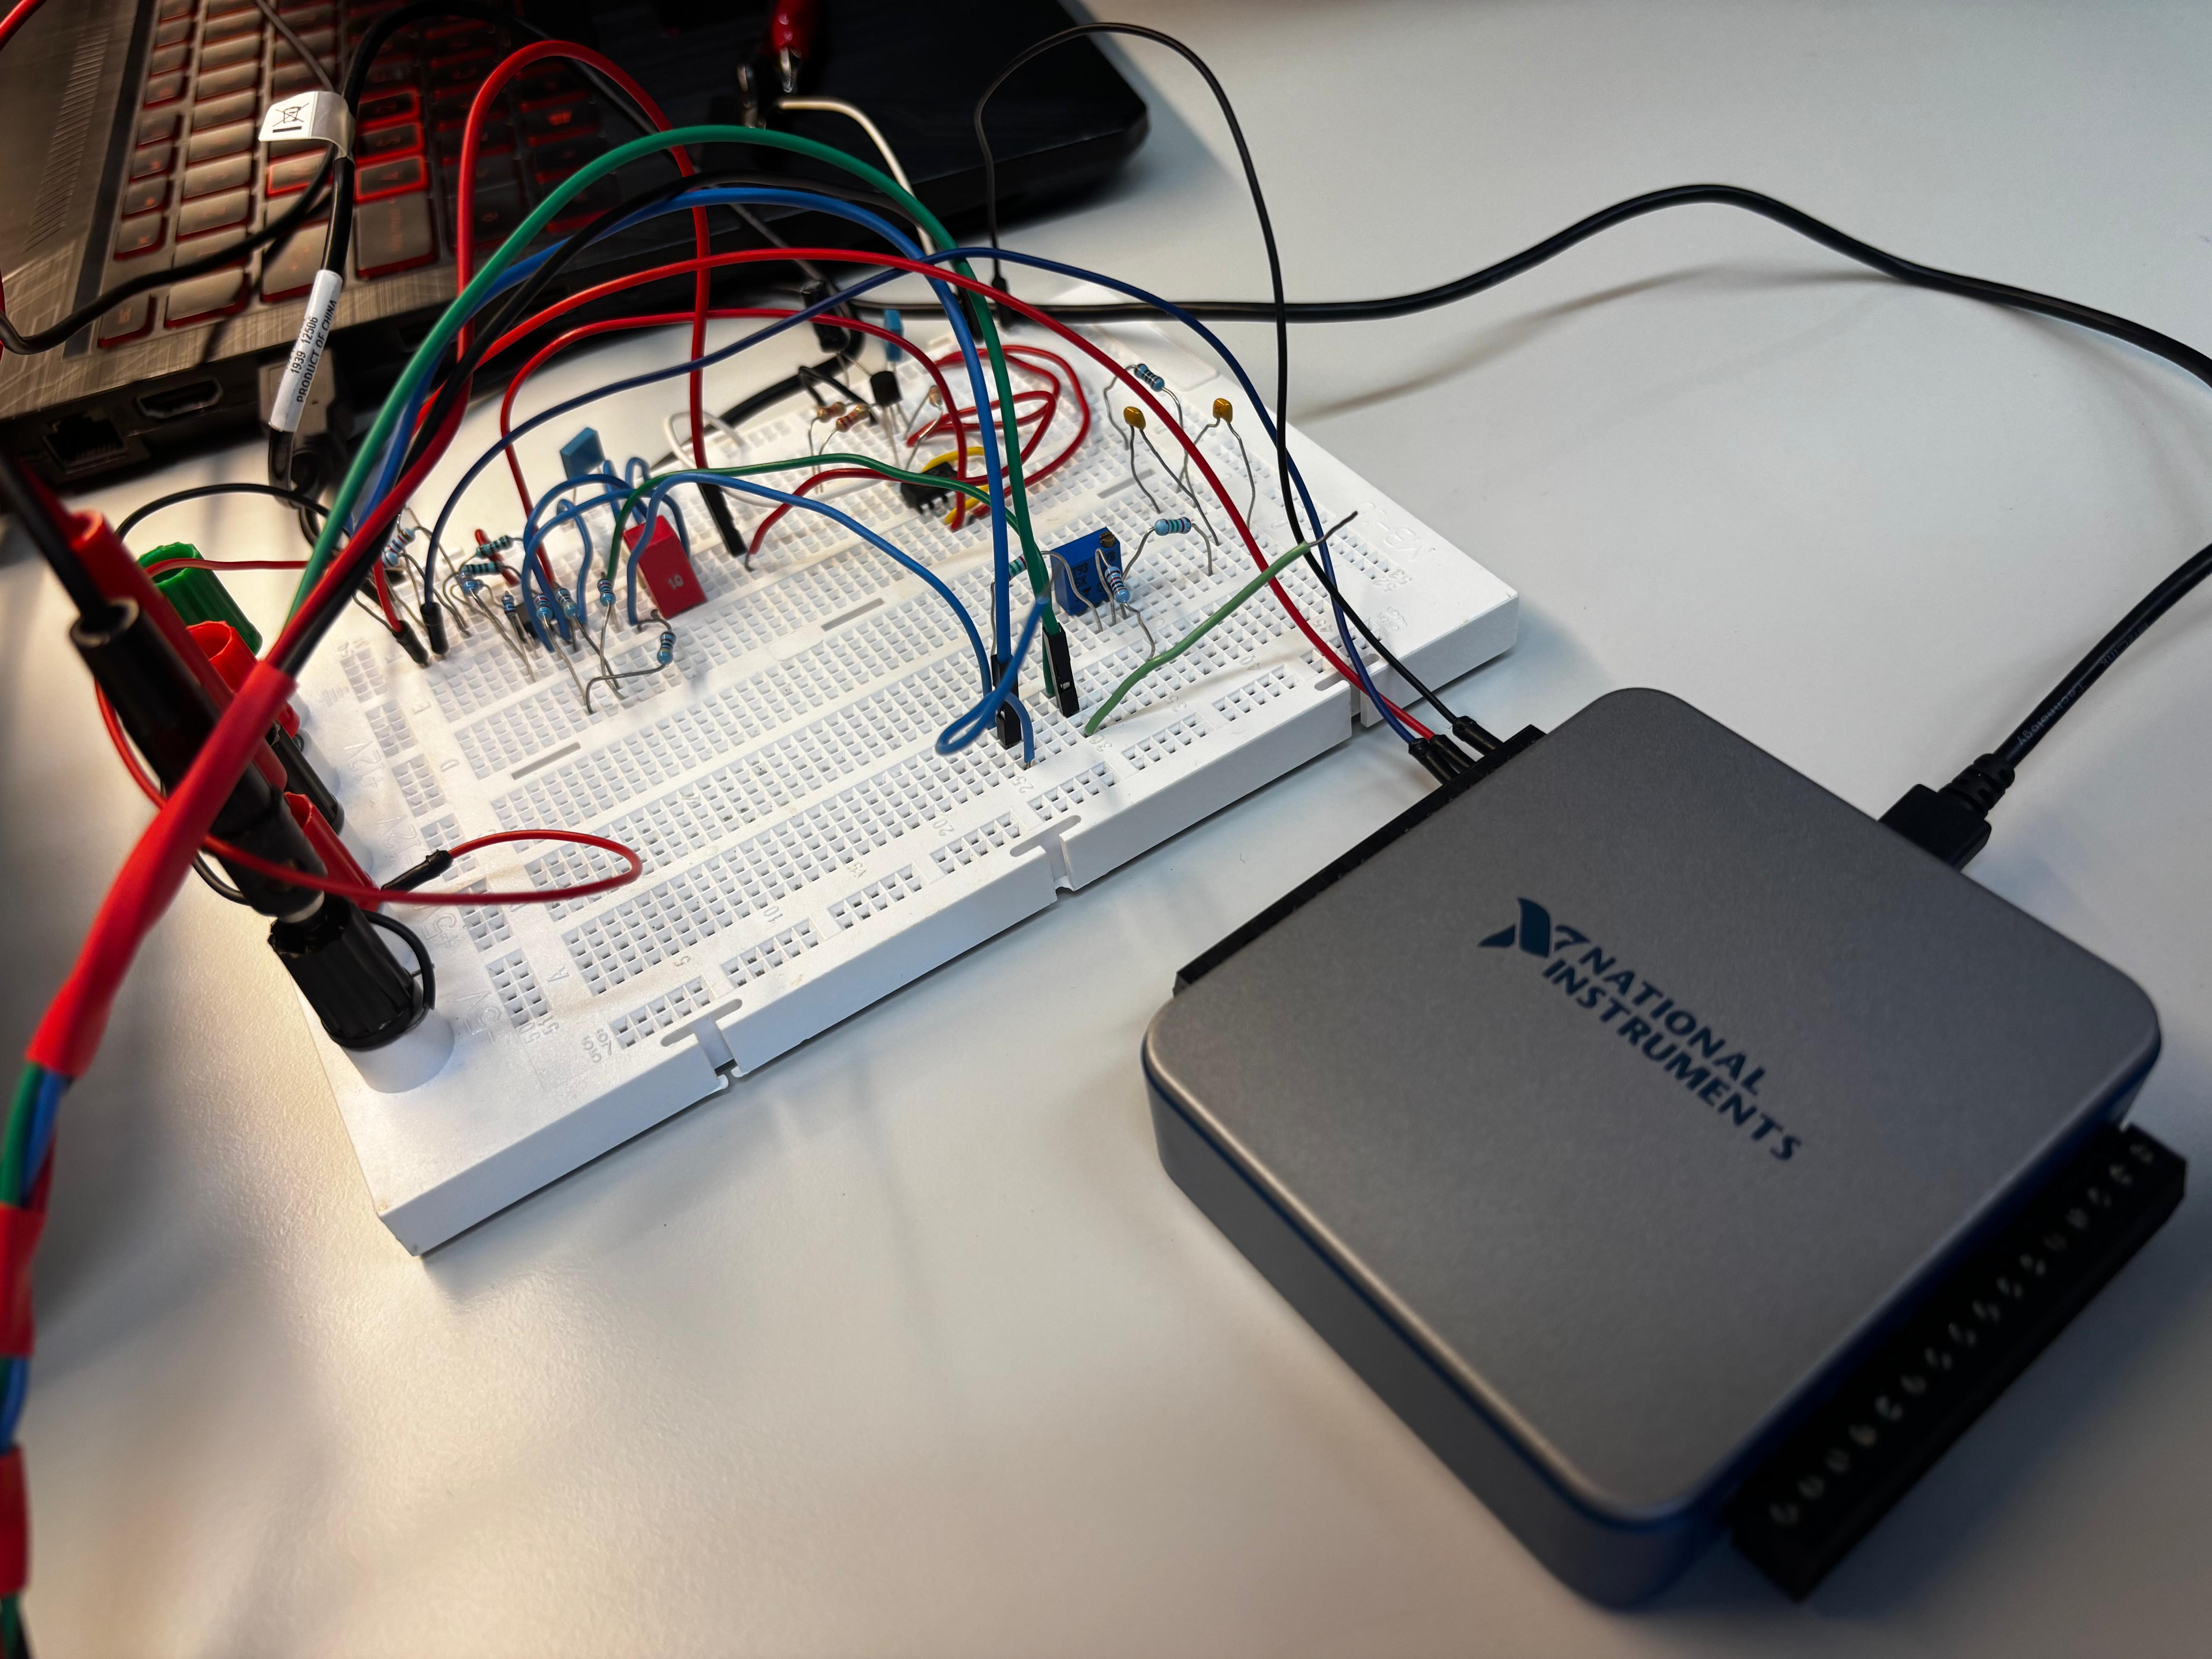
\includegraphics[width=0.65\textwidth]{figs/montaje_final.jpeg}
    \caption{Montaje final.}
    \label{fig:pedestal}
\end{figure}

\section{Conclusiones}
El desarrollo y validación del sistema de pesaje permiten establecer las siguientes conclusiones técnicas:

\begin{enumerate}
    \item La arquitectura implementada, compuesta por la excitación de referencia (objeto a pesar), puente sensor, amplificación de instrumentación, filtrado analógico, adquisición diferencial y procesamiento en \textit{LabVIEW}, permitió materializar una cadena de medida coherente con los requerimientos del informe y funcional en el intervalo experimental de \SIrange{0}{1500}{\g}.

    \item La etapa de acondicionamiento estático cumplió el objetivo de trasladar una señal diferencial del orden de los milivoltios a un nivel utilizable por la DAQ. Con el valor seleccionado de $R_G=\SI{50.2}{\ohm}$ se obtuvo una ganancia aproximada de $G\approx 1993$, lo que condujo a una sensibilidad teórica de alrededor de \SI{1.633}{\milli\V\per\g} y permitió aprovechar de forma segura el rango de entrada del sistema de adquisición.

    \item El pedestal de referencia medido de \SI{1.597}{\V} resultó decisivo para evitar la saturación inferior de la señal analógica. Aunque la tensión en reposo medida de \SI{0.42}{\V} quedó por debajo del intervalo previsto por el análisis de peor caso, el sistema permaneció operativo y la desviación residual pudo ser compensada eficazmente mediante la rutina de tara en \textit{LabVIEW}.

    \item El acondicionamiento dinámico y la adquisición en modo diferencial constituyeron una decisión correcta de diseño. El filtrado de entrada ayudó a limitar interferencias de alta frecuencia sin degradar la banda útil de pesaje, mientras que la lectura diferencial entre AI0 y AI4 redujo la vulnerabilidad frente a ruido en modo común y mantuvo coherencia con la naturaleza diferencial de la señal entregada por la etapa analógica.

    \item La selección de condensadores de poliéster en el filtro de entrada y de condensadores de desacoplo en la excitación de referencia contribuyó de forma directa a la estabilidad eléctrica del sistema. Los primeros ayudaron a conservar el equilibrio de impedancias entre ramas y, con ello, el rechazo de perturbaciones rápidas y de modo común del AD623; los segundos atenuaron transitorios y rizado en la alimentación del puente, evitando que fluctuaciones de la referencia se propagaran como error hacia la medida final.

    \item El análisis conjunto de ruido analógico y cuantización mostró que la limitación inicial del sistema no provenía únicamente del ADC, sino también del ruido de la cadena analógica. La estimación de \SI{470.7}{\micro\V} RMS a la salida y de aproximadamente \SI{3.11}{\milli\V} pico a pico, superior a un LSB de \SI{1.2207}{\milli\V}, justifica técnicamente el promediado digital de 32 muestras como una medida necesaria y no meramente conveniente.

    \item La etapa de procesamiento digital mejoró de manera efectiva la resolución útil del instrumento. Con el promedio de 32 muestras a \SI{128}{\Hz}, el ruido equivalente descendió hasta aproximadamente \SI{83.2}{\micro\V} RMS, lo que lleva la resolución efectiva al entorno de \SI{0.34}{\g} con sensibilidad teórica y \SI{0.35}{\g} con sensibilidad experimental; en consecuencia, el sistema logró una capacidad de discriminación consistente con el objetivo de medición fina dentro del rango ensayado.

    \item La calibración de dos puntos mostró consistencia entre el cálculo manual y la implementación en \textit{LabVIEW}. El factor experimental de \\ \SI{643.42}{\g\per\V} y el valor configurado de  \SI{642.49}{\g\per\V} difieren solo en \SI{0.145}{\percent}, lo que indica que el instrumento virtual reproduce adecuadamente la pendiente de calibración y que los errores de implementación del \textit{software} son pequeños frente al comportamiento global del sistema.

    \item La validación experimental confirmó una respuesta aproximadamente lineal en el intervalo realmente ensayado. A partir de los puntos de \SI{0}{\g}, \SI{1000}{\g} y \SI{1500}{\g}, la máxima desviación absoluta observada fue de \SI{3.46}{\g} y los errores relativos permanecieron por debajo de \SI{0.346}{\percent}.


\end{enumerate}


\bibliographystyle{IEEEtran}
\bibliography{referencias}

\end{document}
